\documentclass[preprint]{sigplanconf}

\usepackage{ifthen}
\usepackage{fancyvrb}
\usepackage{color}
\usepackage{ulem}
\usepackage{xspace}
\usepackage{epsfig}
\usepackage{amssymb}
\usepackage{amsmath}
\usepackage{amsfonts}
\usepackage[utf8]{inputenc}
\usepackage{setspace}

\usepackage{listings}

\usepackage[T1]{fontenc}
\usepackage{beramono}


\definecolor{gray}{rgb}{0.3,0.3,0.3}

\lstset{
  basicstyle=\setstretch{1.1}\ttfamily\footnotesize,
  language=Python,
  keywordstyle=\bfseries,
  stringstyle=\color{blue},
  commentstyle=\color{gray}\textit,
  fancyvrb=true,
  showstringspaces=false,
  %keywords={def,while,if,elif,return,class,get,set,new,guard_class}
}


\newboolean{showcomments}
\setboolean{showcomments}{true}
\ifthenelse{\boolean{showcomments}}
  {\newcommand{\nb}[2]{
    \fbox{\bfseries\sffamily\scriptsize#1}
    {\sf\small$\blacktriangleright$\textit{#2}$\blacktriangleleft$}
   }
   \newcommand{\version}{\emph{\scriptsize$-$Id: main.tex 19055 2008-06-05 11:20:31Z cfbolz $-$}}
  }
  {\newcommand{\nb}[2]{}
   \newcommand{\version}{}
  }

\newcommand\cfbolz[1]{\nb{CFB}{#1}}
\newcommand\arigo[1]{\nb{AR}{#1}}
\newcommand\fijal[1]{\nb{FIJAL}{#1}}
\newcommand\david[1]{\nb{DAVID}{#1}}
\newcommand\anto[1]{\nb{ANTO}{#1}}
\newcommand\reva[1]{\nb{Reviewer 1}{#1}}
\newcommand\revb[1]{\nb{Reviewer 2}{#1}}
\newcommand\revc[1]{\nb{Reviewer 3}{#1}}
\newcommand{\commentout}[1]{}
\newcommand{\ignore}[1]{} % {{\tt \small ignore(#1)}}

\newcommand\ie{i.e.,\xspace}
\newcommand\eg{e.g.,\xspace}
\newcommand{\etal}{\emph{et al.}\xspace}

\normalem

\let\oldcite=\cite

\renewcommand\cite[1]{\ifthenelse{\equal{#1}{XXX}}{[citation~needed]}{\oldcite{#1}}}

%
\def\sharedaffiliation{%
\end{tabular}
\begin{tabular}{c}}
%
\begin{document}
\conferenceinfo{PEPM}{'11, Austin, USA}
\CopyrightYear{2011}
\copyrightdata{[to be supplied]}

\title{Allocation Removal by Partial Evaluation in a Tracing JIT}

\authorinfo{Carl Friedrich Bolz$^a$ \and Antonio Cuni$^a$ \and Maciej Fijałkowski$^b$ \and Michael Leuschel$^a$ \and \\
            Samuele Pedroni$^c$ \and Armin Rigo$^a$}
           {$^a$Heinrich-Heine-Universität Düsseldorf, STUPS Group, Germany

            $^b$merlinux GmbH, Hildesheim, Germany

            $^c$Open End, Göteborg, Sweden
           }
           {cfbolz@gmx.de \and anto.cuni@gmail.com \and fijal@merlinux.eu,
           leuschel@cs.uni-duesseldorf.de \and samuele.pedroni@gmail.com \and arigo@tunes.org}

%\numberofauthors{3}
%\author{
%\alignauthor Carl Friedrich Bolz\\
%       \email{cfbolz@gmx.de}
%\alignauthor Michael Leuschel\\
%       \email{leuschel@cs.uni-duesseldorf.de}
%\alignauthor David Schneider\\
%      \email{david.schneider@uni-duesseldorf.de}
%      \sharedaffiliation
%      \affaddr{Heinrich-Heine-Universität Düsseldorf, STUPS Group, Germany}\\
%}

\maketitle
\begin{abstract}
The performance of many dynamic language implementations suffers from
high allocation rates and runtime type checks.  This makes dynamic
languages less applicable to purely algorithmic problems, despite their
growing popularity.  In this paper, we present a simple optimization
based on online partial evaluation to remove object allocations and
runtime type checks in the context of a tracing JIT.  We evaluate the
optimization using a Python VM and find that it gives good results for
all our (real-life) benchmarks.
\footnote{This research is partially supported by the BMBF funded project PyJIT (nr. 01QE0913B;
Eureka Eurostars).}
\end{abstract}

% A category with the (minimum) three required fields
%\category{H.4}{Information Systems Applications}{Miscellaneous}
%A category including the fourth, optional field follows...
%\category{D.2.8}{Software Engineering}{Metrics}[complexity measures, performance measures]

\category{D.3.4}{Programming Languages}{Processors}[code generation,
interpreters, run-time environments]

\terms
Languages, Performance, Experimentation

\keywords{Tracing JIT, Partial Evaluation, Optimization}

\section{Introduction}

The goal of a just-in-time (JIT) compiler for a dynamic language is obviously to
improve the speed of the language over an implementation of the language that
uses interpretation. The first goal of a JIT is thus to remove the
interpretation overhead, i.e. the overhead of bytecode (or AST) dispatch and the
overhead of the interpreter's data structures, such as operand stack etc. The
second important problem that any JIT for a dynamic language needs to solve is
how to deal with the overhead of boxing of primitive types and of type
dispatching. Those are problems that are usually not present or at least less
severe in statically typed languages.

XXX [fijal] I would say that the other goal of the JIT in case of dynamic
languages is to compile only a common scenario and leave a guard (instead
of proving that something will never ever happen)

Boxing of primitive types is necessary because dynamic languages need to be able to handle
all objects, even integers, floats, booleans etc. in the same way as user-defined
instances. Thus those primitive types are usually \emph{boxed}, i.e. a small
heap-structure is allocated for them, that contains the actual value. Boxing
primitive types can be very costly, because a lot of common operations,
particularly all arithmetic operations, have to produce a new box, in addition
to the actual computation they do. Because the boxes are allocated on the heap,
producing a lot of them puts pressure on the garbage collector.

Type dispatching is the process of finding the concrete implementation that is
applicable to the objects at hand when doing a generic operation on them. An
example would be the addition of two objects: The addition needs to check what
the concrete objects that should be added are, and choose the implementation
that is fitting for them. Type dispatching is a very common operation in a
dynamic language because no types are known at compile time, so all operations
need it.

A recently popular approach to implementing just-in-time compilers for dynamic
languages is that of a tracing JIT. A tracing JIT works by observing the running
program and recording its hot spots into linear execution traces, which are then turned into
machine code. One reason for the popularity of tracing JITs is their relative
simplicity. They can often be added to an interpreter and a lot of the
infrastructure of an interpreter can be reused. They give some important
optimizations like inlining and constant-folding for free. A tracing JIT always
produces linear pieces of code, which simplifies many optimizations that are usually
hard in a compiler, such as register allocation.

The usage of a tracing JIT can remove the overhead of bytecode dispatch and that
of the interpreter data structures. In this paper we want to present a new
optimization that can be added to a tracing JIT that further removes some of the
overhead more closely associated to dynamic languages, such as boxing overhead
and type dispatching. Our experimental platform is the PyPy project, which is an
environment for implementing dynamic programming languages. PyPy and tracing
JITs are described in more detail in Section~\ref{sec:Background}.
Section~\ref{sec:lifetimes} analyzes the problem to be solved more closely.

The core of our trace optimization technique can be
viewed as partial evaluation: the partial evaluation
performs a form of escape analysis \cite{bruno_blanchet_escape_2003} on the traces and make some
objects that are allocated in the trace \emph{static}\footnote{These objects are
called \emph{virtual} in Psyco \cite{rigo_representation-based_2004}.} which
means that they do not occur any more in the optimized trace. This technique is
informally described in Section~\ref{sec:statics}, a more formal description is
given in Section~\ref{sec:formal}.

In Section~\ref{sec:support} we describe some supporting techniques that are not
central to the approach, but are needed to improve the results. The introduced
techniques are evaluated in Section~\ref{sec:Evaluation} using PyPy's Python
interpreter as a case study.

The contributions of this paper are:

\begin{enumerate}
    \item An efficient and effective algorithm for removing object allocations in a tracing JIT.
    \item A characterization of this algorithm as partial evaluation.
    \item A rigorous evaluation of this algorithm.
\end{enumerate}


\section{Background}
\label{sec:Background}

\subsection{PyPy}
\label{sub:PyPy}

The work described in this paper was done in the context of the PyPy project
\cite{armin_rigo_pypys_2006}. PyPy is an environment where dynamic languages can
be implemented in a simple yet efficient way. 
When implementing a language with PyPy one writes an \emph{interpreter}
for the language in
\emph{RPython} \cite{davide_ancona_rpython:_2007}. RPython ("restricted Python")
is a subset of Python chosen in such a way that type inference becomes
possible. The language interpreter can then be compiled (``translated'') with
PyPy's tools into a VM on the C level. Because the interpreter is written at a
relatively high level, the language implementation is kept free of low-level
details, such as object layout, garbage collection or memory model. Those
aspects of the final VM are woven into the generated code during the translation
to C.

A number of languages have been implemented with PyPy. The project was initiated
to get a better Python implementation, which inspired the name of the project
and is still the main focus of development. In addition a number of other
languages were implemented, among them a Prolog interpreter
\cite{carl_friedrich_bolz_towards_2010}, a Smalltalk VM
\cite{carl_friedrich_bolz_back_2008} and a GameBoy emulator
\cite{bruni_pygirl:_2009}.

The feature that makes PyPy more than a compiler with a runtime system is its
support for automated JIT compiler generation \cite{bolz_tracing_2009}. During
the translation to C, PyPy's tools can generate a just-in-time compiler for the
language that the interpreter is implementing. This process is mostly
automatic; it only needs to be guided by the language implementer using a small number of
source-code hints. Mostly-automatically generating a JIT compiler has many advantages
over writing one manually, which is an error-prone and tedious process.
By construction, the generated JIT has the same semantics as the interpreter.
Many optimizations can benefit all languages implemented as an interpreter in RPython.

Moreover, thanks to the internal design of the JIT generator, it is very easy
to add new \emph{backends} for producing the actual machine code, in addition
to the original backend for the Intel \emph{x86} architecture.  Examples of
additional JIT backends are the one for Intel \emph{x86-64} and an
experimental one for the CLI .NET Virtual Machine \cite{cuni_high_2010}.
PyPy's JIT generator generates a \emph{tracing JIT
compiler}, a concept which we now explain in more details.

\subsection{Tracing JIT Compilers}
\label{sub:JIT_background}

Tracing JITs are a recently popular approach to write just-in-time compilers for
dynamic languages. Their origins lie in the Dynamo project, which used a tracing
approach to optimize machine code using execution traces
\cite{bala_dynamo:_2000}. Tracing JITs have then be adapted to be used for a
very light-weight Java VM \cite{gal_hotpathvm:_2006} and afterwards used in
several implementations of dynamic languages, such as JavaScript
\cite{andreas_gal_trace-based_2009}, Lua\footnote{\texttt{http://luajit.org/}}
and now Python (and other languages) via PyPy.

The core idea of tracing JITs is to focus the optimization effort of the JIT
compiler on the hot paths of the core loops of the program and to just use an
interpreter for the less commonly executed parts. VMs that use a tracing JIT are
thus mixed-mode execution environments, they contain both an interpreter and a
JIT compiler. By default the interpreter is used to execute the program, doing
some light-weight profiling at the same time. This profiling is used to identify
the hot loops of the program. If a hot loop is found in that way, the
interpreter enters a special \emph{tracing mode}. In this tracing mode, the
interpreter tries to record all operations that it is executing while running one
iteration of the hot loop. This history of executed operations of one loop is
called a \emph{trace}. Because the trace corresponds to one iteration of a loop,
it always ends with a jump to its own beginning. The trace also contains all
operations that are performed in functions that were called in the loop, thus a
tracing JIT automatically performs inlining.

This trace of operations is then the basis of the generated code. The trace is
first optimized, and then turned into machine code. Both optimization
and machine code generation is simple, because the traces are linear. This
linearity makes many optimizations a lot more tractable, and the inlining that
happens gives the optimizations automatically more context to work with.

Since the trace corresponds to one concrete execution of a loop,
the code generated from it is only one possible path through it.
To make sure that the trace is maintaining the correct semantics, it contains a
\emph{guard} at all places where the execution could have diverged from the
path. Those guards check the assumptions under which execution can stay on the
trace. As an example, if a loop contains an \lstinline{if} statement, the trace
will contain the execution of one of the paths only, which is the path that was
taken during the production of the trace. The trace will also contain a guard
that checks that the condition of the \lstinline{if} statement is true, because if
it isn't, the rest of the trace is not valid.

When generating machine code, every guard is be turned into a quick check to
see whether the assumption still holds. When such a guard is hit during the
execution of the machine code and the assumption does not hold, the execution of
the machine code is stopped, and interpreter continues to run from that point
on. These guards are the only mechanism to stop the execution of a trace, the
loop end condition also takes the form of a guard.

If one specific guard fails often enough, the tracing JIT will generate a new
trace that starts exactly at the position of the failing guard. The existing
assembler is patched to jump to the new trace when the guard fails
\cite{andreas_gal_incremental_2006}.  This approach guarantees that all the
hot paths in the program will eventually be traced and compiled into efficient
code.

\subsection{Running Example}

For the purpose of this paper, we are going to use a tiny interpreter for a dynamic language with
 a very simple object
model, that just supports an integer and a float type. The objects support only
two operations, \lstinline{add}, which adds two objects (promoting ints to floats in a
mixed addition) and \lstinline{is_positive}, which returns whether the number is greater
than zero. The implementation of \lstinline{add} uses classical Smalltalk-like
double-dispatching.
%These classes could be part of the implementation of a very
%simple interpreter written in RPython.
The classes can be seen in
Figure~\ref{fig:objmodel} (written in RPython).

\begin{figure}
\begin{lstlisting}[mathescape]
class Base(object):
   pass

class BoxedInteger(Base):
   def __init__(self, intval):
      self.intval = intval

   def add(self, other):
      return other.add__int(self.intval)

   def add__int(self, intother):
      return BoxedInteger(intother + self.intval)

   def add__float(self, floatother):
      floatvalue = floatother + float(self.intval)
      return BoxedFloat(floatvalue)

   def is_positive(self):
      return self.intval > 0

class BoxedFloat(Base):
   def __init__(self, floatval):
      self.floatval = floatval

   def add(self, other):
      return other.add__float(self.floatval)

   def add__int(self, intother):
      floatvalue = float(intother) + self.floatval
      return BoxedFloat(floatvalue)

   def add__float(self, floatother):
      return BoxedFloat(floatother + self.floatval)

   def is_positive(self):
      return self.floatval > 0.0


def f(y):
   res = BoxedInteger(0)
   while y.is_positive():
      res = res.add(y).add(BoxedInteger(-100))
      y = y.add(BoxedInteger(-1))
   return res
\end{lstlisting}
\caption{An ``Interpreter'' for a Tiny Dynamic Language Written in RPython}
\label{fig:objmodel}
\end{figure}

Using these classes to implement arithmetic shows the basic problem that a
dynamic language implementation has. All the numbers are instances of either
\lstinline{BoxedInteger} or \lstinline{BoxedFloat}, thus they consume space on the
heap. Performing many arithmetic operations produces lots of garbage quickly,
thus putting pressure on the garbage collector. Using double dispatching to
implement the numeric tower needs two method calls per arithmetic operation,
which is costly due to the method dispatch.

To understand the problems more directly, let us consider the simple
interpreter function \lstinline{f} that uses the object model (see the bottom of
Figure~\ref{fig:objmodel}).

The loop in \lstinline{f} iterates \lstinline{y} times, and computes something in the process.
Simply running this function is slow, because there are lots of virtual method
calls inside the loop, one for each \lstinline{is_positive} and even two for each
call to \lstinline{add}. These method calls need to check the type of the involved
objects repeatedly and redundantly. In addition, a lot of objects are created
when executing that loop, many of these objects do not survive for very long.
The actual computation that is performed by \lstinline{f} is simply a sequence of
float or integer additions.


\begin{figure}
\begin{lstlisting}[mathescape]
# arguments to the trace: $p_{0}$, $p_{1}$
# inside f: res.add(y)
guard_class($p_{1}$, BoxedInteger)
    # inside BoxedInteger.add
    $i_{2}$ = get($p_{1}$, intval)
    guard_class($p_{0}$, BoxedInteger)
        # inside BoxedInteger.add__int
        $i_{3}$ = get($p_{0}$, intval)
        $i_{4}$ = int_add($i_{2}$, $i_{3}$)
        $p_{5}$ = new(BoxedInteger)
            # inside BoxedInteger.__init__
            set($p_{5}$, intval, $i_{4}$)

# inside f: BoxedInteger(-100) 
$p_{6}$ = new(BoxedInteger)
    # inside BoxedInteger.__init__
    set($p_{6}$, intval, -100)

# inside f: .add(BoxedInteger(-100))
guard_class($p_{5}$, BoxedInteger)
    # inside BoxedInteger.add
    $i_{7}$ = get($p_{5}$, intval)
    guard_class($p_{6}$, BoxedInteger)
        # inside BoxedInteger.add__int
        $i_{8}$ = get($p_{6}$, intval)
        $i_{9}$ = int_add($i_{7}$, $i_{8}$)
        $p_{10}$ = new(BoxedInteger)
            # inside BoxedInteger.__init__
            set($p_{10}$, intval, $i_{9}$)

# inside f: BoxedInteger(-1)
$p_{11}$ = new(BoxedInteger)
    # inside BoxedInteger.__init__
    set($p_{11}$, intval, -1)

# inside f: y.add(BoxedInteger(-1))
guard_class($p_{0}$, BoxedInteger)
    # inside BoxedInteger.add
    $i_{12}$ = get($p_{0}$, intval)
    guard_class($p_{11}$, BoxedInteger)
        # inside BoxedInteger.add__int
        $i_{13}$ = get($p_{11}$, intval)
        $i_{14}$ = int_add($i_{12}$, $i_{13}$)
        $p_{15}$ = new(BoxedInteger)
            # inside BoxedInteger.__init__
            set($p_{15}$, intval, $i_{14}$)

# inside f: y.is_positive()
guard_class($p_{15}$, BoxedInteger)
    # inside BoxedInteger.is_positive
    $i_{16}$ = get($p_{15}$, intval)
    $i_{17}$ = int_gt($i_{16}$, 0)
# inside f
guard_true($i_{17}$)
jump($p_{15}$, $p_{10}$)
\end{lstlisting}
\caption{Unoptimized Trace for the Simple Object Model}
\label{fig:unopt-trace}
\end{figure}

If the function is executed using the tracing JIT, with \lstinline{y} being a
\lstinline{BoxedInteger}, the produced trace looks like
Figure~\ref{fig:unopt-trace} (lines starting with the hash ``\#'' are comments).

The operations in the trace are shown indented to
correspond to the stack level of the function that contains the traced
operation. The trace is in single-assignment form, meaning that each variable is
assigned to exactly once. The arguments $p_0$ and $p_1$ of the loop correspond
to the live variables \lstinline{y} and \lstinline{res} in the original function.

The operations in the trace correspond to the operations in the RPython program
in Figure~\ref{fig:objmodel}:

\begin{itemize}
    \item \lstinline{new} corresponds to object creation.
    \item \lstinline{get} correspond to attribute reads.
    \item \lstinline{set} correspond to attribute writes.
    \item \lstinline{guard_class} correspond to method calls and are followed by
    the trace of the called method.
    \item \lstinline{int_add} and \lstinline{int_get} are integer addition and
    comparison (``greater than''), respectively.
\end{itemize}

The method calls in the trace are always preceded by a \lstinline{guard_class}
operation, to check that the class of the receiver is the same as the one that
was observed during tracing.\footnote{\lstinline{guard_class} performs a precise
class check, not checking for subclasses.} These guards make the trace specific
to the situation where \lstinline{y} is really a \lstinline{BoxedInteger}, it can
already be said to be specialized for \lstinline{BoxedIntegers}. When the trace is
turned into machine code and then executed with \lstinline{BoxedFloats}, the
first \lstinline{guard_class} instruction will fail and execution will continue
using the interpreter.

The trace shows the inefficiencies of \lstinline{f} clearly, if one looks at the
number of \lstinline{new}, \lstinline{set/get} and \lstinline{guard_class} operations.
In the rest of the paper we will see how this trace can be optimized using
partial evaluation.

XXX add comment that guards are not only slow, but also use lots of memory

\section{Object Lifetimes in a Tracing JIT}
\label{sec:lifetimes}

% section Object Lifetimes in a Tracing JIT (end)

To understand the problems that this paper is trying to solve some more, we
first need to understand various cases of object lifetimes that can occur in a
tracing JIT compiler.

\begin{figure}
\begin{center}
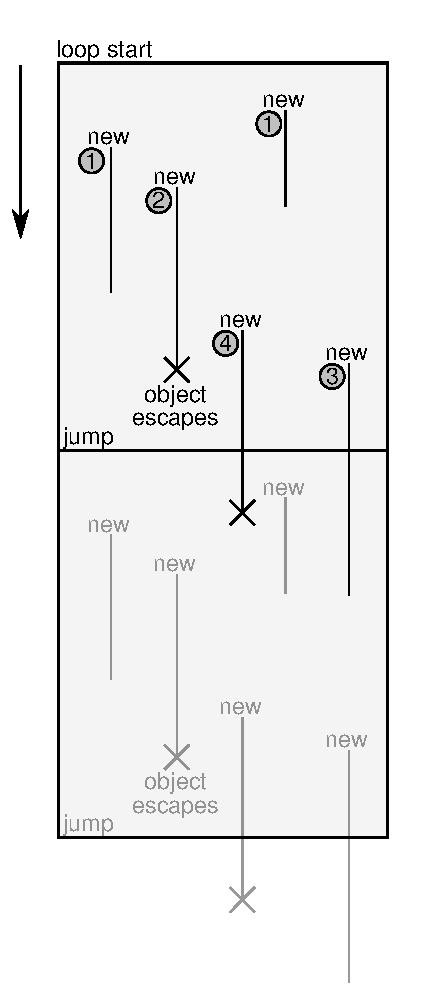
\includegraphics[scale=0.6]{figures/obj-lifetime.pdf}
\end{center}

\caption{Object Lifetimes in a Trace}
\label{fig:lifetimes}
\end{figure}

Figure~\ref{fig:lifetimes} shows a trace before optimization, together with the
lifetime of various kinds of objects created in the trace. It is executed from
top to bottom. At the bottom, a jump is used to execute the same loop another
time (for clarity, the figure shows two iterations of the loop). The loop is
executed until one of the guards in the trace fails, and the execution is
aborted and interpretation resumes.

Some of the operations within this trace are \lstinline{new} operations, which each
create a new instance of some class. These instances are used for a while, e.g.
by calling methods on them (which are inlined into the trace), reading and
writing their fields. Some of these instances \emph{escape}, which means that
they are stored in some globally accessible place or are passed into a
non-inlined function via a residual call.

Together with the \lstinline{new} operations, the figure shows the lifetimes of the
created objects. The objects that are created within a trace using \lstinline{new}
fall into one of several categories:

\begin{itemize}
    \item Category 1: Objects that live for a while, and are then just not
    used any more.

    \item Category 2: Objects that live for a while and then escape.

    \item Category 3: Objects that live for a while, survive across the jump to
    the beginning of the loop, and are then not used any more.

    \item Category 4: Objects that live for a while, survive across the jump,
    and then escape. To these we also count the objects that live across several
    jumps and then either escape or stop being used.
\end{itemize}

The objects that are allocated in the example trace in
Figure~\ref{fig:unopt-trace} fall into categories 1 and 3. Objects stored in
$p_{5}$, $p_{6}$, $p_{11}$ are in category 1, objects in $p_{10}$, $p_{15}$ are in
category 3.

The creation of objects in category 1 is removed by the optimization described
in Sections~\ref{sec:statics} and \ref{sec:formal}. Objects in the other
categories are partially optimized by this approach as well.

\section{Allocation Removal in Traces}
\label{sec:statics}

\subsection{Static Objects}

XXX add a footnote saying that "static" is meant in the sense of PE, not static
allocation

The main insight to improve the code shown in the last section is that objects
in category 1 don't survive very long -- they are used only inside the loop and
nobody else in the program stores a reference to them. The idea for improving
the code is thus to analyze which objects fall in category 1 and thus do
not have to be allocated at all.

This is a process that is usually called \emph{escape analysis}. In this paper we will
perform escape analysis by using partial evaluation. The partial evalution is a
bit peculiar in that it receives no static input arguments for the trace,
but it is only used to optimize operations within a trace.

The partial evaluation works by traversing the trace from beginning to end.
Whenever a \lstinline{new} operation is seen, the operation is removed and a static
object is constructed and associated with the variable that would have stored
the result of \lstinline{new}. The static object describes the shape of the
original object, \eg where the values that would be stored in the fields of the
allocated object come from, as well as the type of the object. Whenever the
optimizer sees a \lstinline{set} that writes into such an object, that shape
description is updated and the operation can be removed, which means that the
operation was done at partial evaluation time. When the optimizer encounters a
\lstinline{get} from such an object, the result is read from the shape
description, and the operation is also removed. Equivalently, a
\lstinline{guard_class} on a variable that has a shape description can be removed
as well, because the shape description stores the type and thus the outcome of
the type check the guard does is statically known.

In the example from last section, the following operations in the upper half
of Fig.~\ref{fig:unopt-trace} would produce two
static objects, and would thus be completely removed from the optimized trace:

\begin{lstlisting}[mathescape,xleftmargin=20pt]
$p_{5}$ = new(BoxedInteger)
set($p_{5}$, intval, $i_{4}$)
$p_{6}$ = new(BoxedInteger)
set($p_{6}$, intval, -100)
\end{lstlisting}


The static object associated with $p_{5}$ would know that it is a
\lstinline{BoxedInteger} whose \lstinline{intval} field contains $i_{4}$; the
one associated with $p_{6}$ would know that it is a \lstinline{BoxedInteger}
whose \lstinline{intval} field contains the constant -100.

The subsequent operations in Fig.~\ref{fig:unopt-trace},
 which use $p_{5}$ and $p_{6}$, could then be
optimized using that knowledge:

\begin{lstlisting}[mathescape,xleftmargin=20pt]
guard_class($p_{5}$, BoxedInteger)
$i_{7}$ = get($p_{5}$, intval)
# inside BoxedInteger.add
guard_class($p_{6}$, BoxedInteger)
# inside BoxedInteger.add__int
$i_{8}$ = get($p_{6}$, intval)
$i_{9}$ = int_add($i_{7}$, $i_{8}$)
\end{lstlisting}

First, the \lstinline{guard_class} operations can be removed, because the classes of $p_{5}$ and
$p_{6}$ are known to be \lstinline{BoxedInteger}. Second, the \lstinline{get} operations can be removed
and $i_{7}$ and $i_{8}$ are just replaced by $i_{4}$ and -100. Thus the only
remaining operation in the optimized trace would be:

\begin{lstlisting}[mathescape,xleftmargin=20pt]
$i_{9}$ = int_add($i_{4}$, -100)
\end{lstlisting}

The rest of the trace from Fig.~\ref{fig:unopt-trace} is optimized similarly.

So far we have only described what happens when static objects are used in guards and in
operations that read and write fields. When the static
object is used in any other operation, it cannot remain static. For example, when
a static object is stored in a globally accessible place, the object has to
be allocated, as it might live longer than one iteration of the loop
and because the partial evaluator looses track of it. This means that the static
object needs to be turned into a dynamic one, \ie lifted. This makes it
necessary to put operations into the residual code that allocate the
static object at runtime.

This is what happens at the end of the trace in Fig.~\ref{fig:unopt-trace}, when the \lstinline{jump} operation
is hit. The arguments of the jump are at this point static objects. Before the
jump is emitted, they are \emph{lifted}. This means that the optimizer produces code
that allocates a new object of the right type and sets its fields to the field
values that the static object has (if the static object points to other static
objects, those need to be lifted as well, recursively). This means that instead of a simple jump,
the following operations are emitted:

\begin{lstlisting}[mathescape,xleftmargin=20pt]
$p_{15}$ = new(BoxedInteger)
set($p_{15}$, intval, $i_{14}$)
$p_{10}$ = new(BoxedInteger)
set($p_{10}$, intval, $i_{9}$)
jump($p_{15}$, $p_{10}$)
\end{lstlisting}

Observe how the operations for creating these two instances have been moved to later point in the
trace. 
At first sight, it may look like for these operations we didn't gain much, as
the objects are still allocated in the end. However, our optimizations were still
worthwhile, because some operations that have been performed
on the lifted static objects have been removed (some \lstinline{get} operations
and \lstinline{guard_class} operations).

\begin{figure}
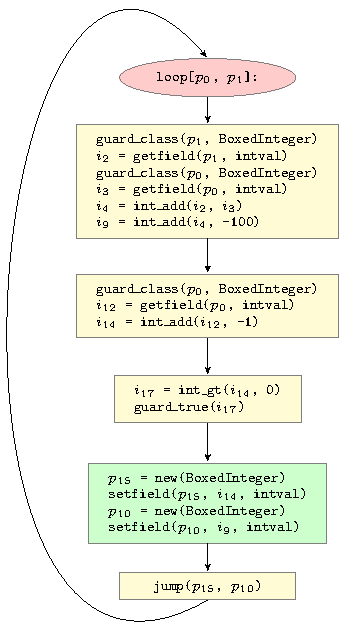
\includegraphics{figures/step1.pdf}
\caption{Resulting Trace After Allocation Removal}
\label{fig:step1}
\end{figure}

The final optimized trace of the example can be seen in Figure~\ref{fig:step1}.
The optimized trace contains only two allocations, instead of the original five,
and only three \lstinline{guard_class} operations, from the original seven.

\section{Formal Description of the Algorithm}
\label{sec:formal}


\begin{figure*}
\begin{center}
\begin{tabular}{lcccc}
\emph{new} & ${\displaystyle \frac{l\,\mathrm{fresh}}{v=\mathtt{new}(T),E,H\overset{\mathrm{run}}{\Longrightarrow}E\left[v\mapsto l\right],H\left[l\mapsto\left(T,\mathrm{null},\mathrm{null}\right)\right]}}$ & ~~~ & \emph{guard} & ${\displaystyle \frac{\mathrm{type}(H(E(v))=T}{\mathtt{guard\_class}(v,T),E,H\overset{\mathrm{run}}{\Longrightarrow}E,H}}$\tabularnewline[3em]
\emph{get} & ${\displaystyle \frac{\,}{u=\mathtt{get}(v,F),E,H\overset{\mathrm{run}}{\Longrightarrow}E\left[u\mapsto H\left(E\left(v\right)\right)_{F}\right],H}}$ & ~~~ &  & ${\displaystyle \frac{\mathrm{type}(H(E(v))\neq T}{\mathtt{guard\_class}(v,T),E,H\overset{\mathrm{run}}{\Longrightarrow}\bot,\bot}}$\tabularnewline[3em]
\emph{set} & ${\displaystyle \frac{\,}{\mathtt{set}\left(v,F,u\right),E,H\overset{\mathrm{run}}{\Longrightarrow}E,H\left[E\left(v\right)\mapsto\left(H\left(E\left(v\right)\right)!_{F}E(u)\right)\right]}}$ & ~~~ &  & \tabularnewline[4em]
\end{tabular}

\begin{minipage}[b]{7 cm}
\emph{Object Domains:}
$$\setlength\arraycolsep{0.1em}
 \begin{array}{rcll}
    u,v & \in & V & \mathrm{\ variables\ in\ trace}\\
    T & \in & \mathfrak{T} & \mathrm{\ runtime\ types}\\
    F & \in & \left\{ L,R\right\} & \mathrm{\ fields\ of\ objects}\\
    l & \in & L & \mathrm{\ locations\ on\ heap}
 \end{array}
$$
\end{minipage}
\begin{minipage}[b]{5 cm}
\emph{Semantic Values:}
$$\setlength\arraycolsep{0.1em}
 \begin{array}{rcll}
    E & \in & V\rightharpoonup L & \mathrm{\ Environment}\\
    H & \in & L\rightharpoonup\mathfrak{T}\times(L\cup \{ \mathrm{null} \})\times (L\cup \{ \mathrm{null}\} ) & \mathrm{\ Heap}\\
    \\
    \\
 \end{array}
$$
\end{minipage}
\end{center}
\caption{The Operational Semantics of Simplified Traces}
\label{fig:semantics}
\end{figure*}

In this section we want to give a formal description of the semantics of the
traces and of the optimizer and liken the optimization to partial evaluation.
We concentrate on the operations for manipulating dynamically allocated objects,
as those are the only ones that are actually optimized. Without loss of
generality we also consider only objects with two fields in this section.

Traces are lists of operations. The operations considered here are \lstinline{new} (to make
a new object), \lstinline{get} (to read a field out of an object), \lstinline{set} (to write a field
into an object) and \lstinline{guard_class} (to check the type of an object). The values of all
variables are locations (i.e.~pointers). Locations are mapped to objects, which
are represented by triples of a type $T$, and two locations that represent the
fields of the object. When a new object is created, the fields are initialized
to null, but we require that they are initialized to a real
location before being read, otherwise the trace is malformed.

We use some abbreviations when dealing with object triples. To read the type of
an object, $\mathrm{type}((T,l_1,l_2))=T$ is used. Reading a field $F$ from an
object is written $(T,l_1,l_2)_F$ which either returns $l_1$ if $F=L$ or $l_2$
if $F=R$. To set field $F$ to a new location $l$, we use the notation
$(T,l_1,l_2)!_Fl$, which yields a new triple $(T,l,l_2)$ if $F=L$ or a new
triple $(T,l_1,l)$ if $F=R$.

Figure~\ref{fig:semantics} shows the operational semantics for traces. The
interpreter formalized there executes one operation at a time. Its state is
represented by an environment $E$ and a heap $H$, which are potentially changed by the
execution of an operation. The environment is a partial function from variables
to locations and the heap is a partial function from locations to objects. Note
that a variable can never be null in the environment, otherwise the trace would
be malformed. The environment could not directly map variables to object,
because several variables can contain a pointer to the \emph{same} object. Thus
the "indirection" is needed to express sharing.

We use the following notation for updating partial functions:
$E[v\mapsto l]$ denotes the environment which is just like $E$, but maps $v$ to
$l$.

The \lstinline{new} operation creates a new object $(T,\mathrm{null},\mathrm{null})$ on the
heap under a fresh location $l$ and adds the result variable to the environment,
mapping it to the new location $l$.

The \lstinline{get} operation reads a field $F$ out of an object, and adds the result
variable to the environment, mapping it to the read location. The heap is
unchanged.

The \lstinline{set} operation changes field $F$ of an object stored at the location that
variable $v$ maps to. The new value of the field is the location in variable
$u$. The environment is unchanged.

The \lstinline{guard_class} operation is used to check whether the object stored at the location
that variable $v$ maps to is of type $T$. If that is the case, then execution
continues without changing heap and environment. Otherwise, execution is
stopped.

\subsection{Optimizing Traces}
\label{sub:formalopt}



\begin{figure*}
\begin{center}
\begin{tabular}{lc}
\emph{new} & ${\displaystyle \frac{v^{*}\,\mathrm{fresh}}{v=\mathtt{new}(T),E,S\overset{\mathrm{opt}}{\Longrightarrow}\left\langle \,\right\rangle ,E\left[v\mapsto v^{*}\right],S\left[v^{*}\mapsto\left(T,\mathrm{null,null}\right)\right]}}$\tabularnewline[3em]
\emph{get} & ${\displaystyle \frac{E(v)\in\mathrm{dom}(S)}{u=\mathtt{get}(v,F),E,S\overset{\mathrm{opt}}{\Longrightarrow}\left\langle \,\right\rangle ,E\left[u\mapsto S(E(v))_{F}\right],S}}$\tabularnewline[3em]
 & ${\displaystyle \frac{E(v)\notin\mathrm{dom}(S)\, u^{*}\,\mathrm{fresh}}{u=\mathtt{get}(v,F),E,S\overset{\mathrm{opt}}{\Longrightarrow}\left\langle u^{*}=\mathtt{get}(E(v),F)\right\rangle ,E\left[u\mapsto u^{*}\right],S}}$\tabularnewline[3em]
\emph{set} & ${\displaystyle \frac{E(v)\in\mathrm{dom}(S)}{\mathtt{set}\left(v,F,u\right),E,S\overset{\mathrm{opt}}{\Longrightarrow}\left\langle \,\right\rangle ,E,S\left[E\left(v\right)\mapsto\left(S(E(v))!_{F}E(u)\right)\right]}}$\tabularnewline[3em]
 & ${\displaystyle \frac{E(v)\notin\mathrm{dom}\left(S\right),\,\left(E(v),S\right)\overset{\mathrm{lift}}{\Longrightarrow}\left(\mathrm{ops},S^{\prime}\right)}{\mathtt{set}\left(v,F,u\right),E,S\overset{\mathrm{opt}}{\Longrightarrow}\mathrm{ops}::\left\langle \mathtt{set}\left(E(v),F,E(u)\right)\right\rangle ,E,S^{\prime}}}$\tabularnewline[3em]
\emph{guard} & ${\displaystyle \frac{E(v)\in\mathrm{dom}(S),\,\mathrm{type}(S(E(v)))=T}{\mathtt{guard\_class}(v,T),E,S\overset{\mathrm{opt}}{\Longrightarrow}\left\langle \,\right\rangle ,E,S}}$\tabularnewline[3em]
 & ${\displaystyle \frac{E(v)\notin\mathrm{dom}(S)\vee\mathrm{type}(S(E(v)))\neq T,\,\left(E(v),S\right)\overset{\mathrm{lift}}{\Longrightarrow}\left(\mathrm{ops},S^{\prime}\right)}{\mathtt{guard\_class}(v,T),E,S\overset{\mathrm{opt}}{\Longrightarrow}\left\langle \mathtt{guard\_class}(E\left(v\right),T)\right\rangle ,E,S^{\prime}}}$\tabularnewline[3em]
\emph{lifting} & ${\displaystyle \frac{v^{*}\notin\mathrm{dom}(S)}{v^{*},S\overset{\mathrm{lift}}{\Longrightarrow}\left\langle \,\right\rangle ,S}}$\tabularnewline[3em]
 & ${\displaystyle \frac{v^{*}\in\mathrm{dom}(S),\,\left(v^{*},S\right)\overset{\mathrm{liftfields}}{=\!=\!\Longrightarrow}\left(\mathrm{ops},S^{\prime}\right)}{v^{*},S\overset{\mathrm{lift}}{\Longrightarrow}\left\langle v^{*}=\mathtt{new}\left(T\right)\right\rangle ::ops,S^{\prime}}}$\tabularnewline[3em]
 & ${\displaystyle \frac{\left(S\left(v^{*}\right)_{L},S\setminus\left\{ v^{*}\mapsto S\left(v^{*}\right)\right\} \right)\overset{\mathrm{lift}}{\Longrightarrow}\left(\mathrm{ops}_{L},S^{\prime}\right),\,\left(S\left(v^{*}\right)_{R},S^{\prime}\right)\overset{\mathrm{lift}}{\Longrightarrow}\left(\mathrm{ops}_{R},S^{\prime\prime}\right)}{v^{*},S\overset{\mathrm{liftfields}}{=\!=\!\Longrightarrow}\mathrm{ops}_{L}::ops_{R}::\left\langle \mathtt{set}\left(v^{*},L,S\left(v^{*}\right)_{L}\right),\,\mathtt{set}\left(v^{*},R,S\left(v^{*}\right)_{R}\right)\right\rangle ,S^{\prime}}}$\tabularnewline[3em]
\end{tabular}

\begin{minipage}[b]{7 cm}
\emph{Object Domains:}
$$\setlength\arraycolsep{0.1em}
 \begin{array}{rcll}
    u,v & \in & V & \mathrm{\ variables\ in\ trace}\\
    u^*,v^* & \in & V^* & \mathrm{\ variables\ in\ optimized\ trace}\\
    T & \in & \mathfrak{T} & \mathrm{\ runtime\ types}\\
    F & \in & \left\{ L,R\right\} & \mathrm{\ fields\ of\ objects}\\
 \end{array}
$$
\end{minipage}
\begin{minipage}[b]{5 cm}
\emph{Semantic Values:}
$$\setlength\arraycolsep{0.1em}
 \begin{array}{rcll}
    E & \in & V\rightharpoonup V^* & \mathrm{\ Environment}\\
    S & \in & V^*\rightharpoonup\mathfrak{T}\times(V^*\cup \{ \mathrm{null} \})\times (V^*\cup \{ \mathrm{null}\} ) & \mathrm{\ Static\ Heap}\\
    \\
    \\
 \end{array}
$$
\end{minipage}
\end{center}
\caption{Optimization Rules}
\label{fig:optimization}
\end{figure*}

To optimize the simple traces from the last section, we use online partial
evaluation. The partial evaluator optimizes one operation of the trace at a
time. Every operation in the unoptimized trace is replaced by a list of
operations in the optimized trace. This list is empty if the operation
can be optimized away (which hopefully happens often). The optimization rules
can be seen in Figure~\ref{fig:optimization}.

The state of the optimizer is stored in an environment $E$ and a \emph{static
heap} $S$. The environment is a partial function from variables in the
unoptimized trace $V$ to variables in the optimized trace $V^*$ (which are
themselves written with a
$\ ^*$ for clarity). The reason for introducing new variables in the optimized
trace is that several variables that appear in the unoptimized trace can turn
into the same variables in the optimized trace. Thus the environment of the
optimizer serves a function similar to that of the environment in the semantics: sharing.

The static heap is a partial function from $V^*$ into the
set of static objects, which are triples of a type and two elements of $V^*$.
A variable $v^*$ is in the domain of the static heap $S$ as long as the
optimizer can fully keep track of the object. The image of $v^*$ is what is
statically known about the object stored in it, \ie its type and its fields. The
fields of objects in the static heap are also elements of $V^*$ (or null, for
short periods of time).

When the optimizer sees a \lstinline{new} operation, it optimistically removes it and
assumes that the resulting object can stay static. The optimization for all
further operations is split into two cases. One case is for when the
involved variables are in the static heap, which means that the operation can be
performed at optimization time and removed from the trace. These rules mirror
the execution semantics closely. The other case is for when not enough is known about
the variables, and the operation has to be residualized.

If the argument $v$ of a \lstinline{get} operation is mapped to something in the static
heap, the \lstinline{get} can be performed at optimization time. Otherwise, the \lstinline{get}
operation needs to be residualized.

If the first argument $v$ to a \lstinline{set} operation is mapped to something in the
static heap, then the \lstinline{set} can performed at optimization time and the static heap
updated. Otherwise the \lstinline{set} operation needs to be residualized. This needs to be
done carefully, because the new value for the field, from the variable $u$,
could itself be static, in which case it needs to be lifted first.

If a \lstinline{guard_class} is performed on a variable that is in the static heap, the type check
can be performed at optimization time, which means the operation can be removed
if the types match. If the type check fails statically or if the object is not
in the static heap, the \lstinline{guard_class} is residualized. This also needs to
lift the variable on which the \lstinline{guard_class} is performed.

Lifting takes a variable that is potentially in the static heap and makes sure
that it is turned into a dynamic variable. This means that operations are
emitted that construct an object with the shape described in the
static heap, and the variable is removed from the static heap.

Lifting a static object needs to recursively lift its fields. Some care needs to
be taken when lifting a static object, because the structures described by the
static heap can be cyclic. To make sure that the same static object is not lifted
twice, the \lstinline{liftfield} operation removes it from the static heap \emph{before}
recursively lifting its fields.


% subsection Optimizing Traces (end)

\subsection{Analysis of the Algorithm}
\label{sub:analysis}

While we do not offer a formal proof of it, it should be relatively clear
that the algorithm presented above is sound: it works by delaying (and
often completely removing) some operations.  The algorithm runs in a
single pass over the list of operations.  We can check that altough
recursively lifting a static object is not a constant-time operation,
the algorithm only takes a total time linear in the length of the trace.
Moreover, it gives the ``best'' possible result within its constrains,
\eg in term of the number of residual operations.  The
algorithm itself is not particularly complex or innovative; our focus is
rather that \emph{in the context of tracing JITs} it is possible to find a
simple enough algorithm that still gives the best results.

Note in particular that objects in category 1 (\ie the ones that do
not escape) are completely removed; moreover, objects in category 2
(\ie escaping) are still partially dealt with: if such an object
escapes later than its creation point, all the operations inbetween that
involve the object are removed.

The optimization is particularly effective for chains of operations.
For example, it is typical for an interpreter to generate sequences of
writes-followed-by-reads, where one interpreted opcode writes to some
object's field and the next interpreted opcode reads it back, possibly
dispatching on the type of the object created just before.  In the case
of PyPy's Python interpreter, this optimization can even remove the
allocation of all intermediate frames that occur in the interpreter,
corresponding to all calls that have been inlined in the trace.

% subsection Analysis of the Algorithm (end)

% section Formal Description of the Algorithm (end)

%___________________________________________________________________________

% section Escape Analysis in a Tracing JIT (end)

\section{Supporting Techniques}
\label{sec:support}

\subsection{Virtualizables}
\label{sub:Virtualizables}

\cfbolz{probably can be cut in case of space problems}

One problem to the successful application of the allocation removal techniques
described in the previous sections is the presence of frame-introspection
features in many dynamic languages. Languages such as Python and Smalltalk allow
the programmer to get access to the frames object that the interpreter uses to
store local variables. This is a useful feature, as makes the implementation of
a debugger possible in Python without needing much support from the VM level. On
the other hand, it severely hinders the effectiveness of allocation removal,
because every time an object is stored into a local variable, it is stored into
the frame-object, which makes it escape.

This problem is solved by making it possible to the interpreter author to add
some hints into the source code to declare instances of one class as frame
objects. The JIT will then fill these objects only lazily when they are actually
accessed (\eg because a debugger is used). Therefore in the common case, nothing
is stored into the frame objects, making the problem of too much escaping go
away. This is a common approach in VM implementations \cite{miranda_context_1999}, the only
novelty in our approach lays in its generality, because most other JITs are just
specifically written for one particular language.

% subsection Virtualizables (end)

% section Supporting Techniques (end)

\section{Evaluation}
\label{sec:Evaluation}

To evaluate the effectiveness of our allocation removal algorithm, we look at
the effectiveness when used in the tracing JIT of PyPy's Python interpreter. The
benchmarks we used are small-to-medium Python programs, some synthetic
benchmarks, some real applications.

Some of them are from the Computer Language Benchmark
Game\footnote{\texttt{http://shootout.alioth.debian.org/}}: \textbf{fannkuch},
\textbf{nbody}, \textbf{meteor-contest}, \textbf{spectral-norm}.

Furthermore there are the following benchmarks:
\begin{itemize}
    \item \textbf{crypto\_pyaes}: AES implementation.
    \item \textbf{django}: The templating engine of the Django web
    framework\footnote{\texttt{http://www.djangoproject.com/}}.
    \item \textbf{go}: A Monte-Carlo Go
    AI\footnote{\texttt{http://shed-skin.blogspot.com/2009/07/ disco-elegant-python-go-player.html}}.
    \item \textbf{html5lib}: An HTML5 parser.
    \item \textbf{pyflate-fast}: A BZ2 decoder.
    \item \textbf{raytrace-simple}: A ray tracer.
    \item \textbf{richards}: The Richards benchmark.
    \item \textbf{spambayes}: A Bayesian spam filter\footnote{\texttt{http://spambayes.sourceforge.net/}}.
    \item \textbf{telco}: A Python version of the Telco decimal
    benchmark\footnote{\texttt{http://speleotrove.com/decimal/telco.html}},
    using a pure Python decimal floating point implementation.
    \item \textbf{twisted\_names}: A DNS server benchmark using the Twisted networking
    framework\footnote{\texttt{http://twistedmatrix.com/}}.
\end{itemize}

We evaluate the allocation removal algorithm along two lines: first we want to
know how many allocations could be optimized away. On the other hand, we want
to know how much the run times of the benchmarks is improved.

The benchmarks were run on an otherwise idle Intel Core2 Duo P8400 processor
with 2.26 GHz and 3072 KB of cache on a machine with 3GB RAM running Linux
2.6.35. We compared the performance of various Python implementations on the
benchmarks. As a baseline, we used the standard Python implementation in C,
CPython 2.6.6\footnote{\texttt{http://python.org}}, which uses a bytecode-based
interpreter. Furthermore we compared against Psyco 1.6
\cite{rigo_representation-based_2004}, an extension to CPython which is a
just-in-time compiler that produces machine code at run-time. It is not based
on traces. Finally, we used two versions of PyPy's Python interpreter (revision
77823 of SVN trunk\footnote{\texttt{https://codespeak.net/svn/pypy/trunk}}): one
including the JIT but not optimizing the traces, and one using the allocation
removal optimizations (as well as some minor other optimizations, such as
constant folding).

As the first step, we counted the occurring operations in all generated traces
before and after the optimization phase for all benchmarks. The resulting
numbers can be
seen in Figure~\ref{fig:numops}. The optimization removes as many as 90\% and as
little as 4\% percent of allocation operations in the traces of the benchmarks.
All benchmarks taken together, the optimization removes 70\% percent of
allocation operations. The numbers look similar for reading and writing of
attributes. There are even more \lstinline{guard} operations that are removed,
however there is an additional optimization that removes guards, so not all the
removed guards are an effect of the optimization described here.

\begin{figure*}
\begin{center}
\begin{tabular}{|l||r|rr|rr|rr|rr|}
\hline
	&num loops	&new	&removed	&get/set	&removed &guard &removed	&all ops	&removed\\
\hline
crypto\_pyaes	&78	&3088	&50\%	&57148	&25\%	&9055	&95\%	&137189	&80\%\\
django	&51	&673	&54\%	&19318	&18\%	&3876	&93\%	&55682	&85\%\\
fannkuch	&43	&171	&49\%	&886	&63\%	&1159	&81\%	&4935	&45\%\\
go	&517	&12234	&76\%	&200842	&21\%	&53138	&90\%	&568542	&84\%\\
html5lib	&498	&14432	&68\%	&503390	&11\%	&71592	&94\%	&1405780	&91\%\\
meteor-contest	&59	&277	&36\%	&4402	&31\%	&1078	&83\%	&12862	&68\%\\
nbody	&13	&96	&38\%	&443	&69\%	&449	&78\%	&2107	&38\%\\
pyflate-fast	&162	&2278	&55\%	&39126	&20\%	&8194	&92\%	&112857	&80\%\\
raytrace-simple	&120	&3118	&59\%	&91982	&15\%	&13572	&95\%	&247436	&89\%\\
richards	&87	&844	&4\%	&49875	&22\%	&4130	&91\%	&133898	&83\%\\
spambayes	&314	&5608	&79\%	&117002	&11\%	&25313	&94\%	&324125	&90\%\\
spectral-norm	&38	&360	&64\%	&5553	&20\%	&1122	&92\%	&11878	&77\%\\
telco	&46	&1257	&90\%	&37470	&3\%	&6644	&99\%	&98590	&97\%\\
twisted-names	&214	&5273	&84\%	&100010	&10\%	&23247	&96\%	&279667	&92\%\\
\hline
total	&2240	&49709	&70\%	&1227447	&14\%	&222569	&93\%	&3395548	&89\%\\
\hline
\end{tabular}
\end{center}
\caption{Number of Operations and Percentage Removed By Optimization}
\label{fig:numops}
\end{figure*}

In addition to the count of operations we also performed time measurements.
All benchmarks were run 50 times in the same process, to give the JIT time to produce machine
code. The arithmetic mean of the times of the last 30 runs were used as the
result. The errors were computed using a confidence interval with a 95\%
confidence level \cite{georges_statistically_2007}. The results are reported in Figure~\ref{fig:times}.
With the optimization turned on, PyPy's Python interpreter outperforms CPython
in all benchmarks except spambayes (which heavily relies on regular expression
performance and thus is not helped much by our Python JIT) and meteor-contest.
All benchmarks are improved by the allocation removal optimization, some as much
as XXX. XXX Psyco

XXX runtimes of the algorithm somehow?

\begin{figure*}
\begin{center}
\begin{tabular}{|l||r|r|r|r|}
\hline
	&Cpython	&Psyco	&PyPy w/o optimizations	&PyPy w/ optimizations \\
\hline
crypto\_pyaes	&2757.80 $\pm$ 0.98	&67.90 $\pm$ 0.47	&1652.00 $\pm$ 4.00 &266.86 $\pm$ 5.94 \\
django	&993.19 $\pm$ 0.50	&913.51 $\pm$ 4.22	&694.73 $\pm$ 2.86 &259.53 $\pm$ 1.79 \\
fannkuch	&1987.22 $\pm$ 2.02	&944.44 $\pm$ 0.61	&566.99 $\pm$ 1.06 &466.87 $\pm$ 1.85 \\
go	&947.21 $\pm$ 1.58	&445.96 $\pm$ 0.68	&2197.71 $\pm$ 25.21 &316.15 $\pm$ 9.33 \\
html5lib	&13987.12 $\pm$ 19.51	&17398.25 $\pm$ 36.50	&27194.45 $\pm$ 46.62	&10092.19 $\pm$ 23.50 \\
meteor-contest	&346.98 $\pm$ 0.35	&215.66 $\pm$ 0.23	&433.04 $\pm$ 1.45 &392.85 $\pm$ 0.87 \\
nbody\_modified	&637.90 $\pm$ 1.82	&256.78 $\pm$ 0.18	&135.55 $\pm$ 0.33 &103.93 $\pm$ 0.25 \\
pyflate-fast	&3169.35 $\pm$ 1.89	&1278.16 $\pm$ 3.13	&3285.89 $\pm$ 8.51	&1822.36 $\pm$ 11.52 \\
raytrace-simple	&2744.60 $\pm$ 51.72	&1072.66 $\pm$ 1.08	&2778.27 $\pm$ 15.13	&647.24 $\pm$ 5.44 \\
richards	&354.06 $\pm$ 1.00	&63.48 $\pm$ 0.15	&383.93 $\pm$ 3.28 &88.32 $\pm$ 0.91 \\
spambayes	&299.16 $\pm$ 0.35	&338.68 $\pm$ 3.14	&580.90 $\pm$ 24.68 &397.37 $\pm$ 10.60 \\
spectral-norm	&478.63 $\pm$ 0.80	&139.83 $\pm$ 1.54	&353.51 $\pm$ 1.39 &112.10 $\pm$ 1.17 \\
telco	&1207.67 $\pm$ 2.03	&730.00 $\pm$ 2.66	&1296.08 $\pm$ 4.37 &495.23 $\pm$ 2.14 \\
twisted\_names	&9.58 $\pm$ 0.01	&10.43 $\pm$ 0.01	&17.99 $\pm$ 0.27	&7.13 $\pm$ 0.09 \\
\hline
\end{tabular}
\end{center}
\caption{Benchmark Times in Milliseconds}
\label{fig:times}
\end{figure*}

\section{Related Work}
\label{sec:related}

There exists a large number of works on escape analysis, which is an program
analysis that tries to find an upper bound for the lifetime of objects allocated
at specific program points
\cite{goldberg_higher_1990,park_escape_1992,choi_escape_1999,bruno_blanchet_escape_2003}.
This information can then be used to decide that certain objects can be
allocated on the stack, because their lifetime does not exceed that of the stack
frame it is allocated in. The difference to our work is that escape analysis is
split into an analysis and an optimization phase. The analysis can be a lot more
complex than our simple one-pass optimization. Also, stack-allocation reduces
garbage-collection pressure but does not optimize away the actual accesses to
the stack-allocated object. In our case, an object is not needed at all any
more.
XXX more papers?

Chang \etal describe a tracing JIT for JavaScript running on top of a JVM
\cite{mason_chang_efficient_2007}. They mention in passing an approach to
allocation removal that moves the allocation of an object of type 1 out of the
loop to only allocate it once, instead of every iteration. No details are given
for this optimization. The fact that the object is still allocated and needs to
be written to means that only the allocations are optimized away, but not the
reads and writes out of/into the object.

SPUR, a tracing JIT for C\# seems to be able to remove allocations in a similar
way to the approach described here, as hinted at in the technical report
\cite{michael_bebenita_spur:_2010}. However, no details for the approach and its
implementation are given.

partial evaluation:

Prolog:
partially static datastructures are already built-in to Prolog and was built-into partial
evaluation from the beginning \cite{lloyd_partial_1991}.
 FP

partially static data structures: kenichi asai's thesis?

xxx: relation to compile-time garbage collection \cite{mazur_practical_2001};  separation logic; John Hughes: type specialization


\section{Conclusion}
\label{sec:conclusion}

In this paper, we used an approach based on online partial evaluation to
optimize away allocations in the traces of a tracing JIT.  In this context a
simple approach to partial evaluation gives good results.  This is due
to the fact that the tracing JIT itself is responsible for all control
issues, which are usually the hardest part of partial evaluation: the
tracing JIT selects the parts of the program that are worthwhile to
optimize, and extracts linear paths through them, inlining functions as
necessary.  What is left to optimize is only those linear paths.

We expect a similar result for other optimizations that usually require
a complex analysis phase and are thus normally too slow to use at
runtime.  A tracing JIT selects interesting linear paths by itself;
therefore, a naive version of many optimizations on such paths should
give mostly the same results.  For example, we experimented with (and
plan to write about) store-load propagation with a very simple alias
analysis.


\section*{Acknowledgements}

The authors would like to thank Stefan Hallerstede, David Schneider and Thomas
Stiehl for fruitful discussions during the writing of the paper.

\bibliographystyle{abbrv}
\bibliography{paper}

\end{document}
